
ضخامت غشا از مرتبه‌ی چند نانومتر است و مقیاس انحنا‌هایی که شکل کلی غشا را مشخص می‌کنند از مرتبه‌ی بزرگی میکرون بوده. در نتیجه به طور عمومی مدل کردن شکل و انحنای غشا با یک رویه‌ی ۲ بعدی کاملا قابل قبول است. تصاویر میکروسکوپی غشا مانند شکل‌های 
\ref{fig:budding}
و
\ref{fig:flucmem} 
نشان می‌دهد که غشا سطحی نسبتا صاف و پیوسته دارد. در نتیجه در مقیاس‌های میکرومتری غشا را با رویه‌ای با چنین ویژگی‌ای مدل می‌کنیم. البته که این فرض در مقیاس نانومتری پابرجا نیست. 

\begin{figure}[t]
\begin{center}
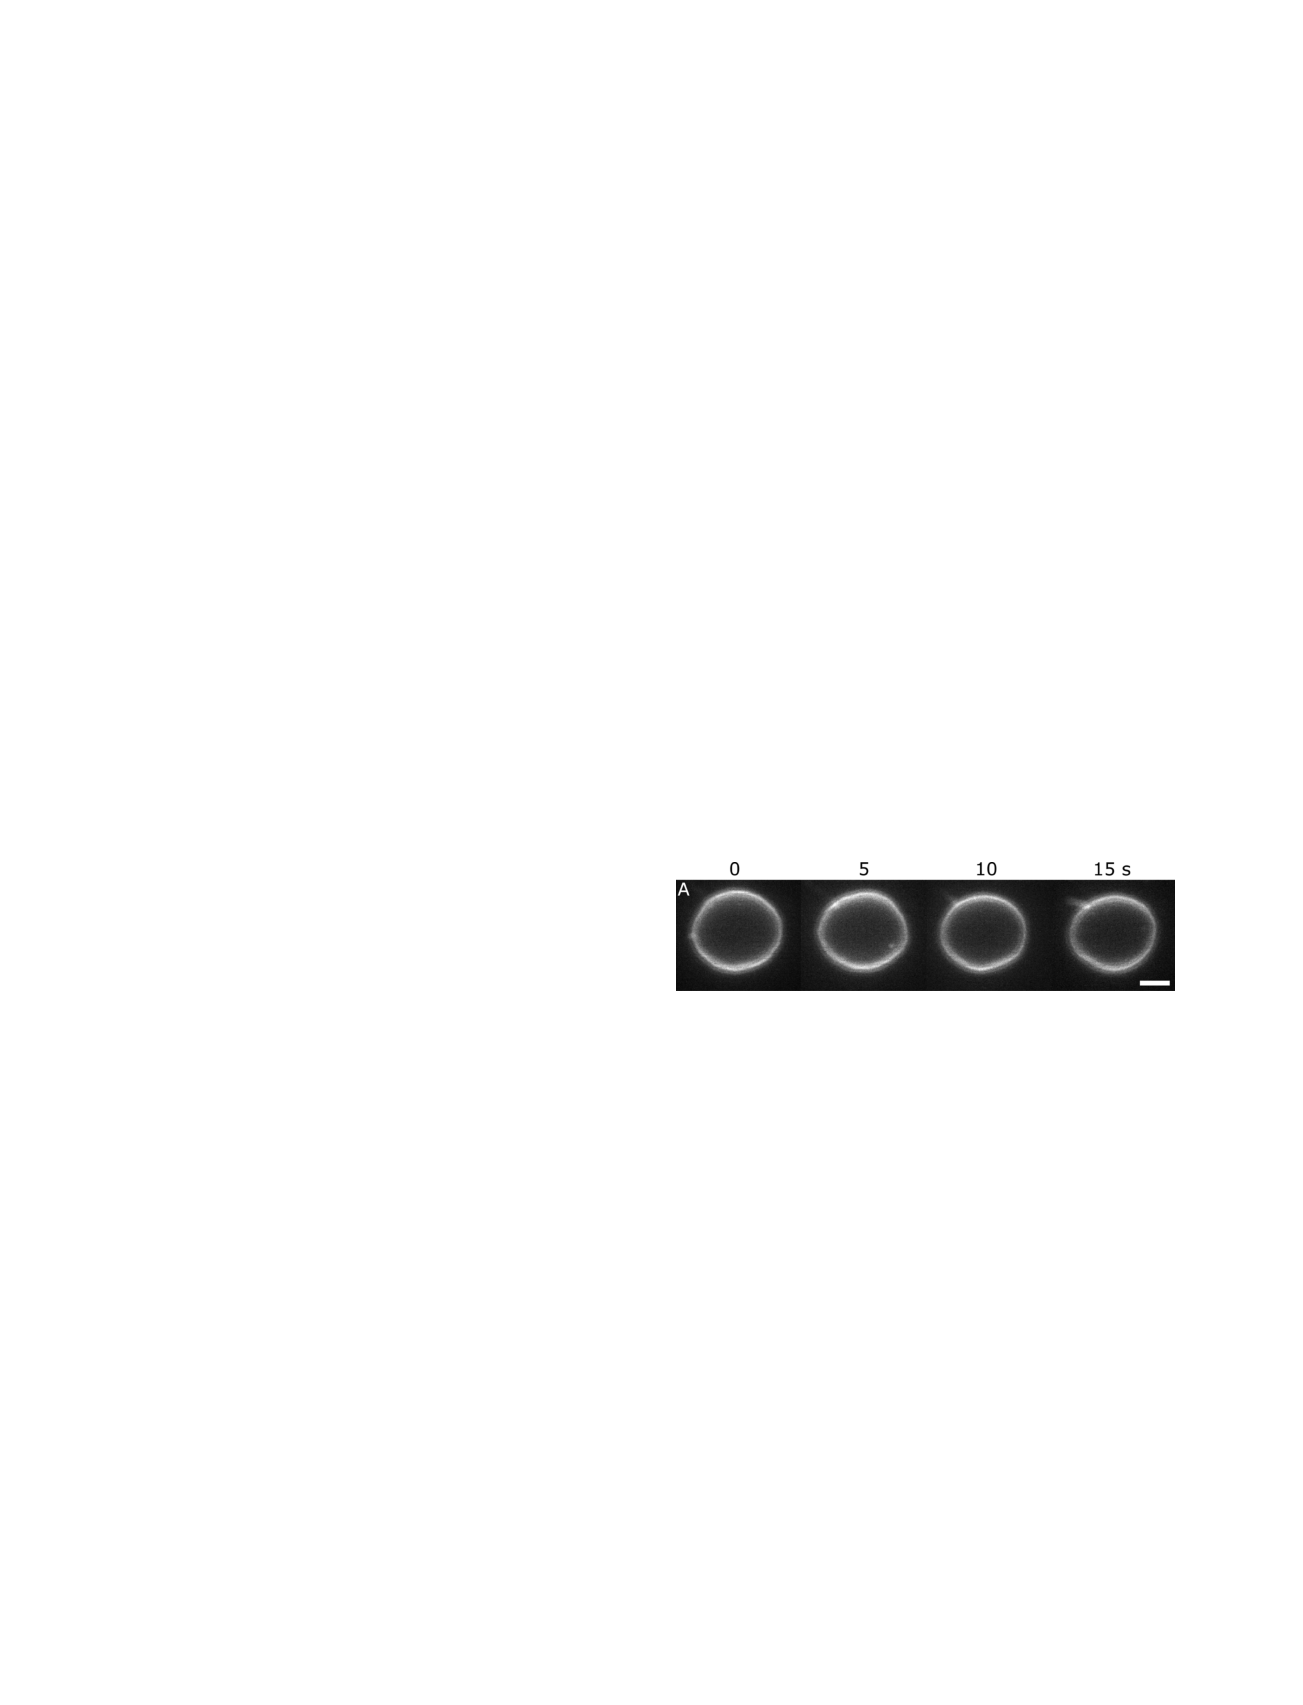
\includegraphics[width=\columnwidth]{\Mempath/Pics/Membrane_fluctuations}
\caption{
مجموعه تصاویر پست سر هم از تغییر شکل یک غشای لیپیدی را با تصویر برداری فلورسانت در بازه‌های ۵ ثانیه‌ای نشان می‌دهد. خط مقیاس سفید رنگ اندازه‌ی ۵ میکرومتر را نشان می‌دهد. 
\cite{ParthasarathyMembraneMeasurement}
}
\label{fig:flucmem}
\end{center}
\end{figure}

مولکول‌های غشا درون یک سیال غوطه‌ور است. مولکول‌ها تحت افت خیز ترمودینامیکی محیط، در جهت‌ درون-صفحه‌ای سطح غشا و جهت عمود بر آن در حال حرکت است. در نتیجه برای تعریف انحنا، لازم است  سطح غشا به بخش‌های کوچک تقسیم بندی شود و با میانگین‌گیری بر روی  مکان مولکول‌ها انحنا را تعیین کرد. اندازه‌ی این بخش‌ها تابع شدت افت و خیز مولکول‌هاست. محاسبات حاصل از  شبیه‌ سازی دینامیک ملکلولی برای غشایی که مولکول‌های یکسان دارد حدود
$5.1$ 
 برابر ضخامت غشا گزارش شده است
\cite{Goetz1998}.
 انحنای هر بخش از یک غشای ساده با ضخامت 
$4nm$,
 حاصل از رفتار دست جمعی حدود 
$100$
مولکول لیپیدی خواهد بود. در مقیاس بزرگ، هر کدام از این بخش‌ها تنها یک نقطه بر روی رویه‌ی غشا را تشکیل می‌دهند. ما می‌توانیم برای هر نقطه روی غشا یک صغحه‌ی مماس و یک صفحه‌ی عمود بر مماس تعریف کنیم. صفحه‌ی عمود بر سطح با رویه‌ی غشا فصل مشترکی به شکل یک خط دارد (مانند شکل 
\ref{fig:normalPlaneIntersection}).
\begin{figure}[h]
\begin{center}
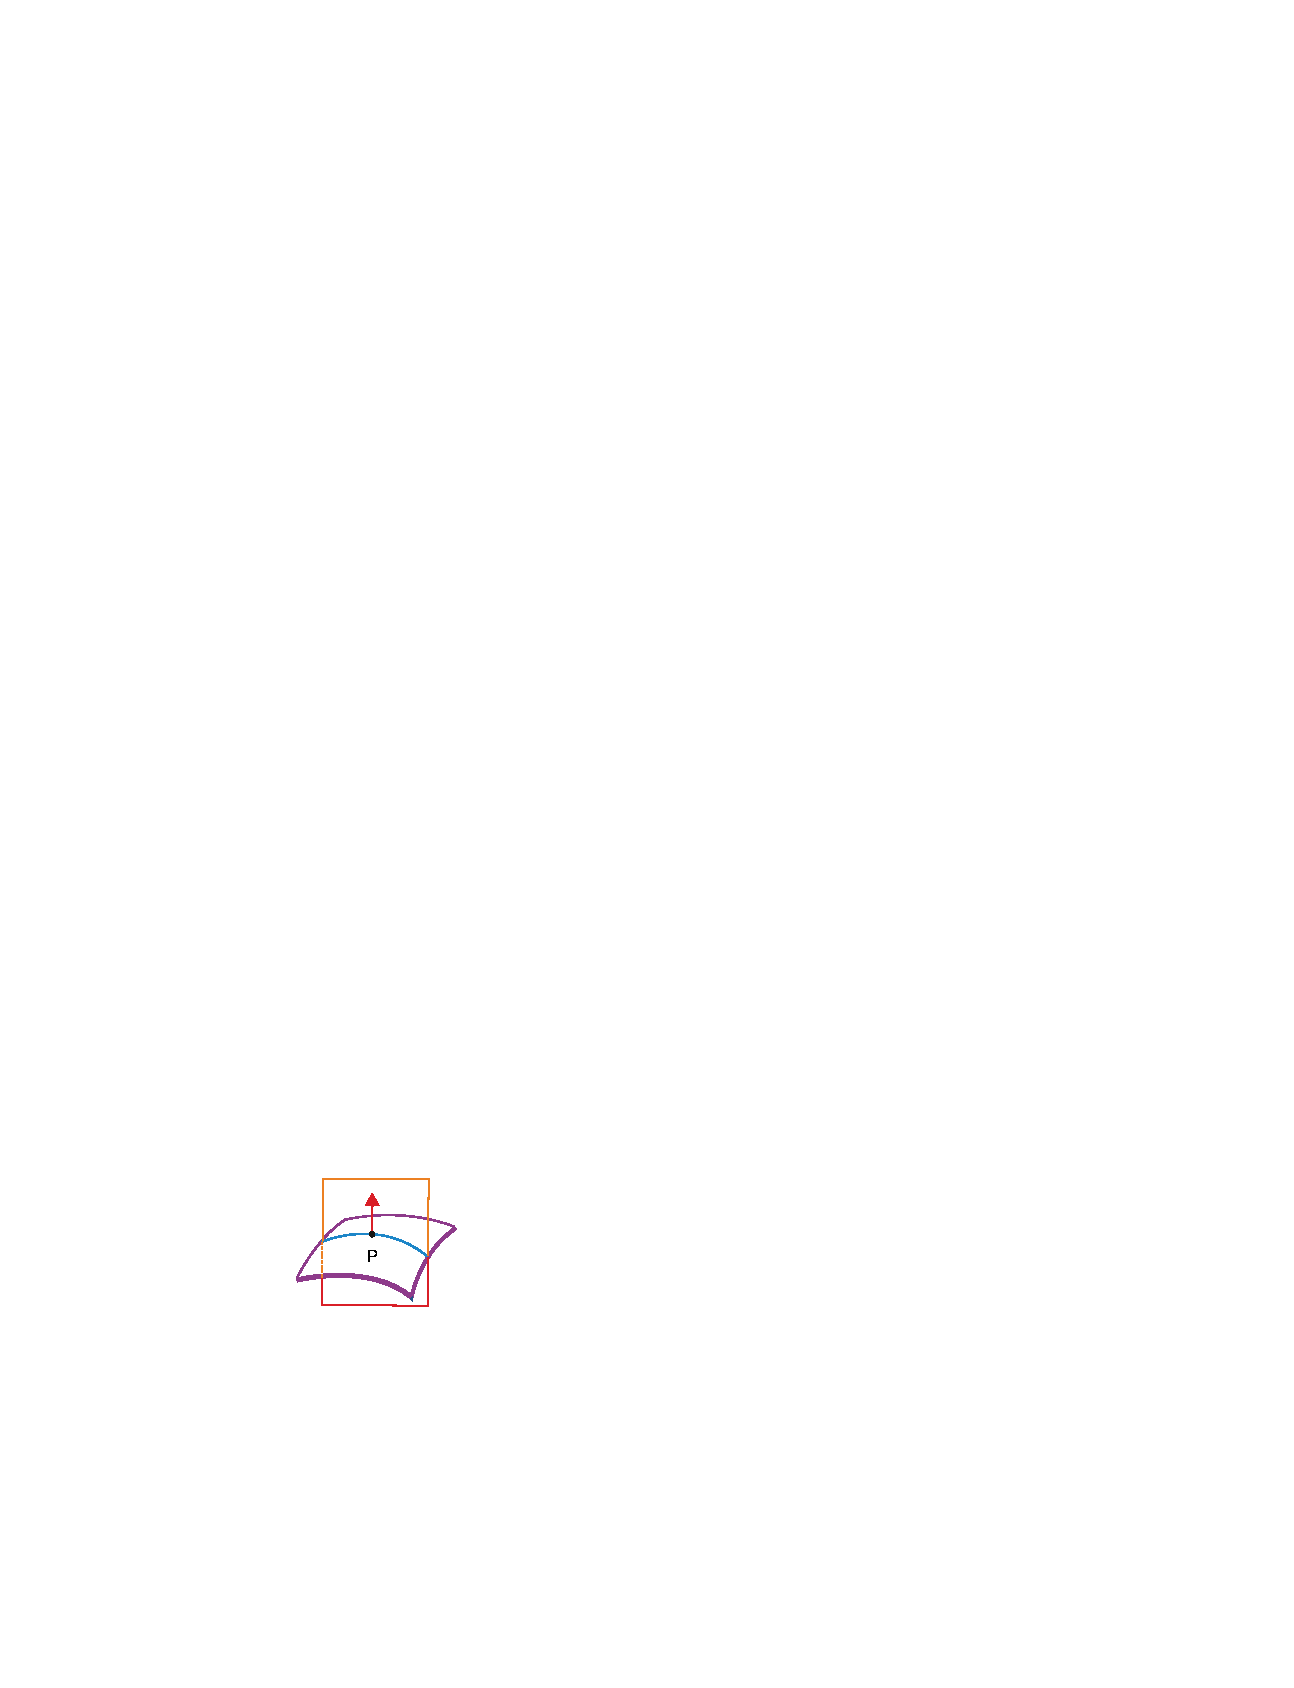
\includegraphics[width=6in]{\MemTB/Pics/NormalPlane}
\caption{
خم حاصل از فصل مشترک صفحه‌ی عمود بر سطح غشا در نقطه‌ی 
P
را نشان می‌دهد.
}
\label{fig:normalPlaneIntersection}
\end{center}
\end{figure}
انحنای تشکیل شده زد فصل مشترک، 
$C$
 در صورتی که در جهت بردار عمود بر سطح باشد 
($\cap$)
 با علامت مثبت و در حالتی که در جهت مخالف باشد 
($\cup$)
 با علامت منفی تعریف می‌شود. می‌توان فرض کرد که خط مشترک قسمتی از یک دایره  است و انحنای این خط عکس شعاع آن دایره خواهد بود. تنها یک  صفحه‌ مماس بر سطح  می‌توان تعریف کرد ولی صفحه‌ی عمود بر سطح می‌تواند در جهت‌های مختلف تعریف شود. انتخاب جهت صفحه‌ی عمود مقدار انحنای محاسبه شده را تغییر خواهد داد. اگر تمام انحناهای ممکن در یک نقطه‌ را با تغییر جهت صفحه‌ی متعامد اندازه‌گیری کنیم، مقادیر در بازه‌ای محدود به  کمینه و بیشینه‌ی انحنا قرار خواهد گرفت،
$C_{min}$
و
$C_{max}$.
 مقادیر کمینه و بیشینه انحنا به انحناهای اصلی سطح معرف هستند که با 
$C_1$
و
$C_2$
نمایش داده می‌شوند. انحناهای اصلی همچنین  ویژه‌مقدار‌های تانسور انحنا در آن نقطه هستند. همچنین اگر انحناهای اصلی برابر یکدیگر نباشند،
$C_1\neq C_2$ 
صفحاتی که خم‌ها با آن تعریف می‌شوند حتما عمود بر هم خواهند بود. از آنجایی که مولکول‌های سطح غشا حرکت پخشی می‌کنند  شکل غشا باید بر اساس تعاریفی باشد که تحت تغییر روش پارامتریزه\LTRfootnote{paprameterisation}  
 کردن سطح ناوردا باشد. انحناهای اصلی سطح چنین ویژگی دارند. انحنای میانگین در هر نقطه‌ بر روی سطح به صورت 
\begin{equation}
M=\frac{1}{2}(C_1+C_2)
\label{eq:meanCurv}
\end{equation}
و انحنای گاووسی به صورت
\begin{equation}
G=C_1C_2
\label{eq:gaussianCurv}
\end{equation}
 تعریف کرد. انحنای میانگین، معادل رَد\LTRfootnote{trace} 
 تانسور انحنا و انحنای گاووسی برابر با دترمینان این تانسور است. همچنین می‌توان روابط بالا را بازنویسی کرد و انحناهای اصلی را بر حسب انحنای میانگین و انحنای گاووسی محاسبه کرد،

\begin{figure}[t]
\begin{center}
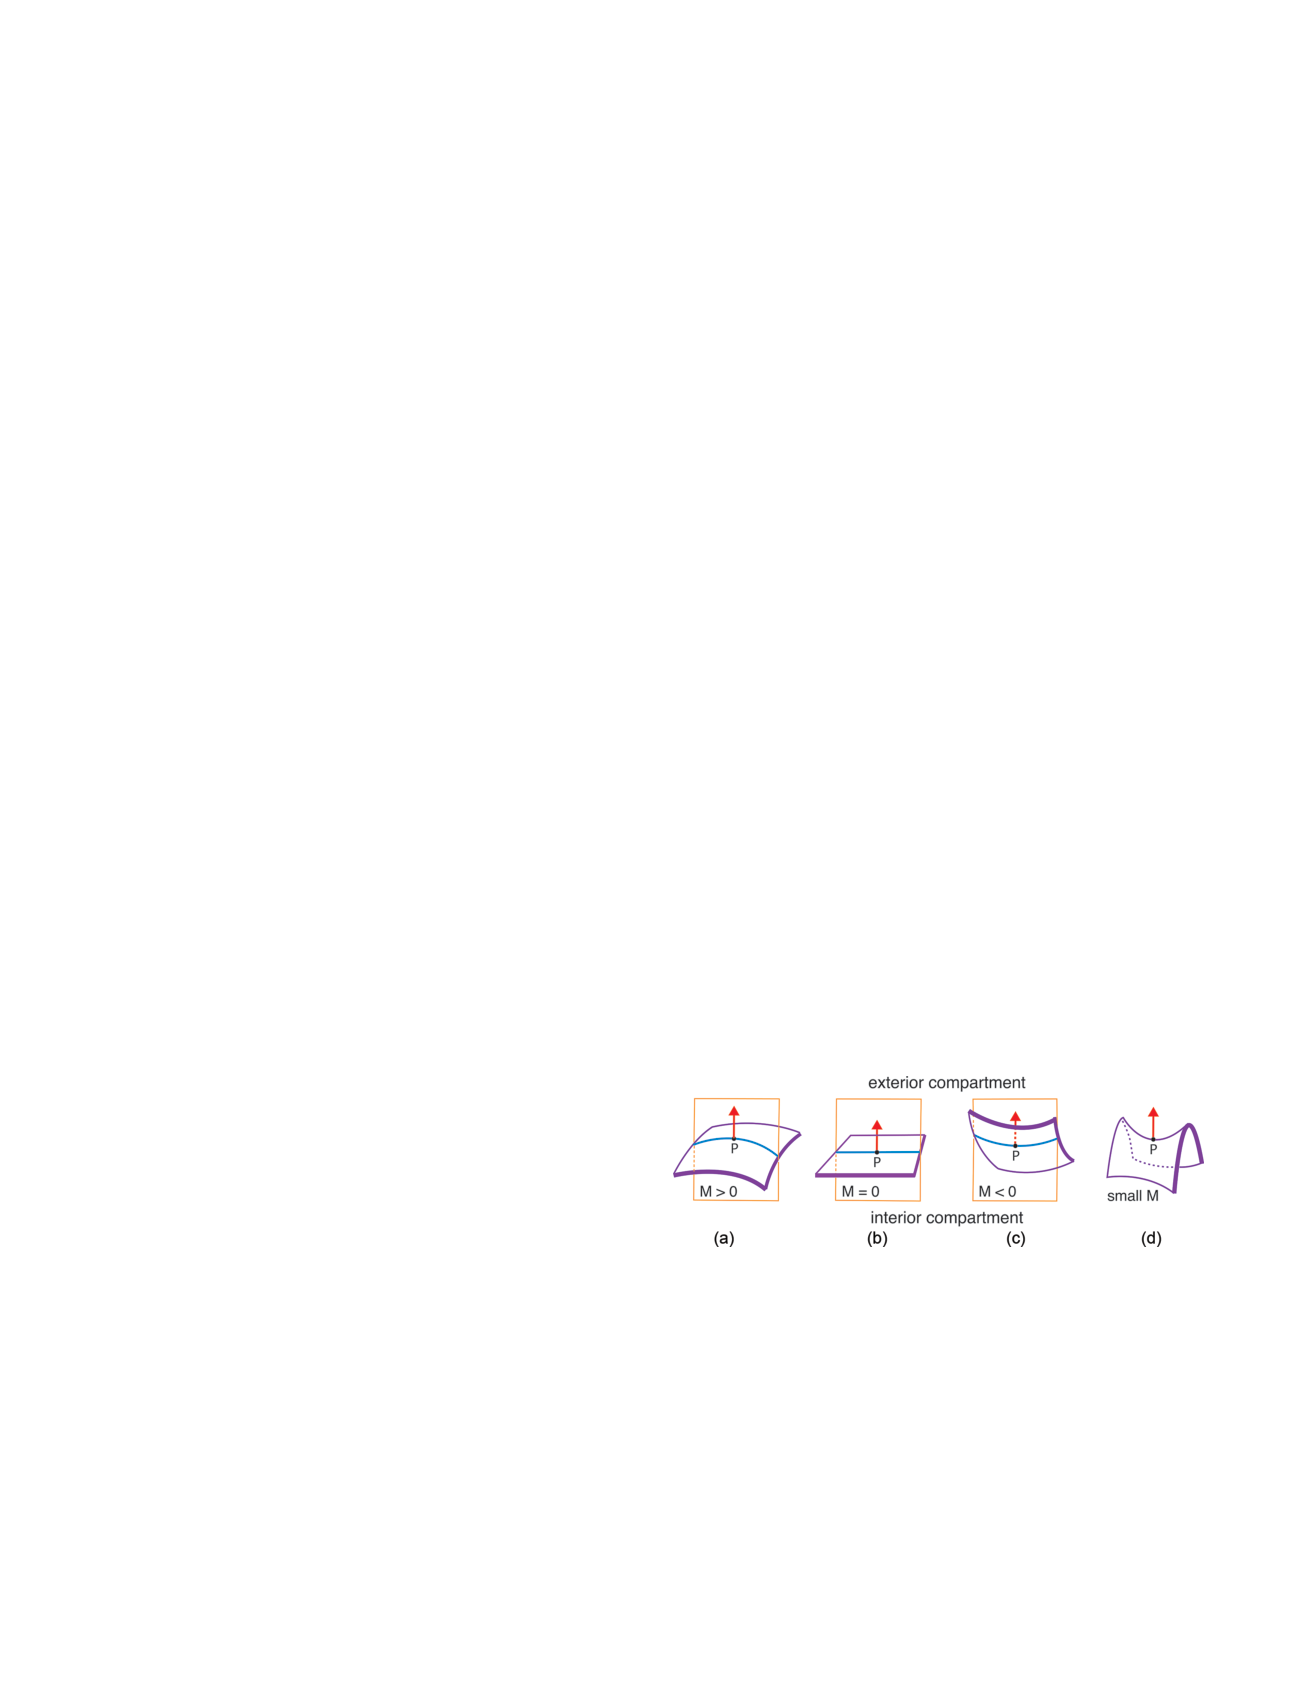
\includegraphics[width=\columnwidth]{\MemTB/Pics/curvatureSign}
\caption{
قرارداد برای تعیین علامت انحنای میانگین. با فرض اینکه بالا محیط خارج غشا و پایین داخل غشا را مشخص کند، بردار نرمال غشا جهت (بردار قرمز رنگ) رو به بالا خواهد داشت. در شکل الف) انحنای میانگین مثبت هنگامی که هر دو انحنای اصلی برآمدگی در جهت بردار نرمال داشته باشند. ب) برای قسمت تخت انحنای میانگین صفر، ج) انحنای منفی هنگامی که  برآمدگی به سمت داخل غشا باشد، د) در نقاط زین اسبی انحناهای اصلی علامت‌های مخالف یکدیگر دارند و در این صورت انحنای میانگین مقدار کمی خواهد داشت.
}
\label{fig:curvatureSign}
\end{center}
\end{figure}

\begin{equation}
\begin{aligned}
C_1&=M-\sqrt{M^2-G}\\
C_2&=M+\sqrt{M^2-G}.
\label{eq:gaussianCurv}
\end{aligned}
\end{equation}
که در روابط بالا، از آنجایی که 
$M^2\geq G$
\cite{Seifert1991}
 هر دو مقدار همیشه حقیقی هستند. مقدار انحنای میانگین، 
 $M$،
 تحت تمامی تبدیل‌های دستگاه مختصات که دترمینان ژاکوبین آن مثبت باشد (جهت بردار عمود بر سطح را تغییر ندهد) تغییر نخواهد کرد. به طور مثال اگر یک سطح با پارامتر‌های 
 $(s^1,s^2)$
 تعریف شده باشد، تبدیلی که پارامتر‌ها را با یکدیگر تعویض کند، 
 $(s^{-1}\equiv s^2,s^{-2}\equiv s^1)$
 تبدیلی است که جهت نرمال سطح را تغییر می‌دهد که در نتیجه علامت انحنای میانگین را تغییر می‌دهد. هرچند که چنین تبدیل‌هایی در فیزیک بسیار مهم هستند زیرا که انتخاب دستگاه مختصات بر مشخصات برخی خواص فیزیکی نباید تاثیرگذار باشد، ولی در مورد انحنا باید تعریف مشخصی برای محاسبات وجود داشته باشد تا بتوان میان محیط داخل و خارج غشا تمییز قائل بشویم. با توجه به رابطه‌ی
 \ref{eq:meanCurv}
 علامت انحنای میانگین در هر نقطه روی غشا تابع مقادیر انحناهای اصلی در آن نقطه‌ است. شکل 
 \ref{fig:curvatureSign}
 حالت‌های مختلف که بر علامت انحنای میانگین تاثیر می‌گذارد را نشان می‌دهد. 

به طور کلی، برای سطح تخت انحنای میانگین صفر است، در صورتی که برآمدگی انحنا به سمت داخل غشا باشد، انحنای میانگین منفی و در صورتی که برآمدگی به سمت بیرون غشا باشد، انحنای میانگین مثبت خواهد بود. در نقاط زین اسبی انحناهای اصلی علامت‌های مخالف یکدیگر دارند و در نتیجه مقدار انحنای میانگین بسیار کوچک خواهد بود. مهم است که اشاره شود که انحنای میانگین ابزار مناسبی برای اندازه‌گیری تاثیر نقاط زین اسبی نیست زیراکه مقدار آن با سطح تخت اختلاف چندانی ندارد. برای اندازه‌گیری تاثیر نقاط زین اسبی، انحنای گاووسی ابزار مناسبی است.
\begin{figure}[t]
\begin{center}
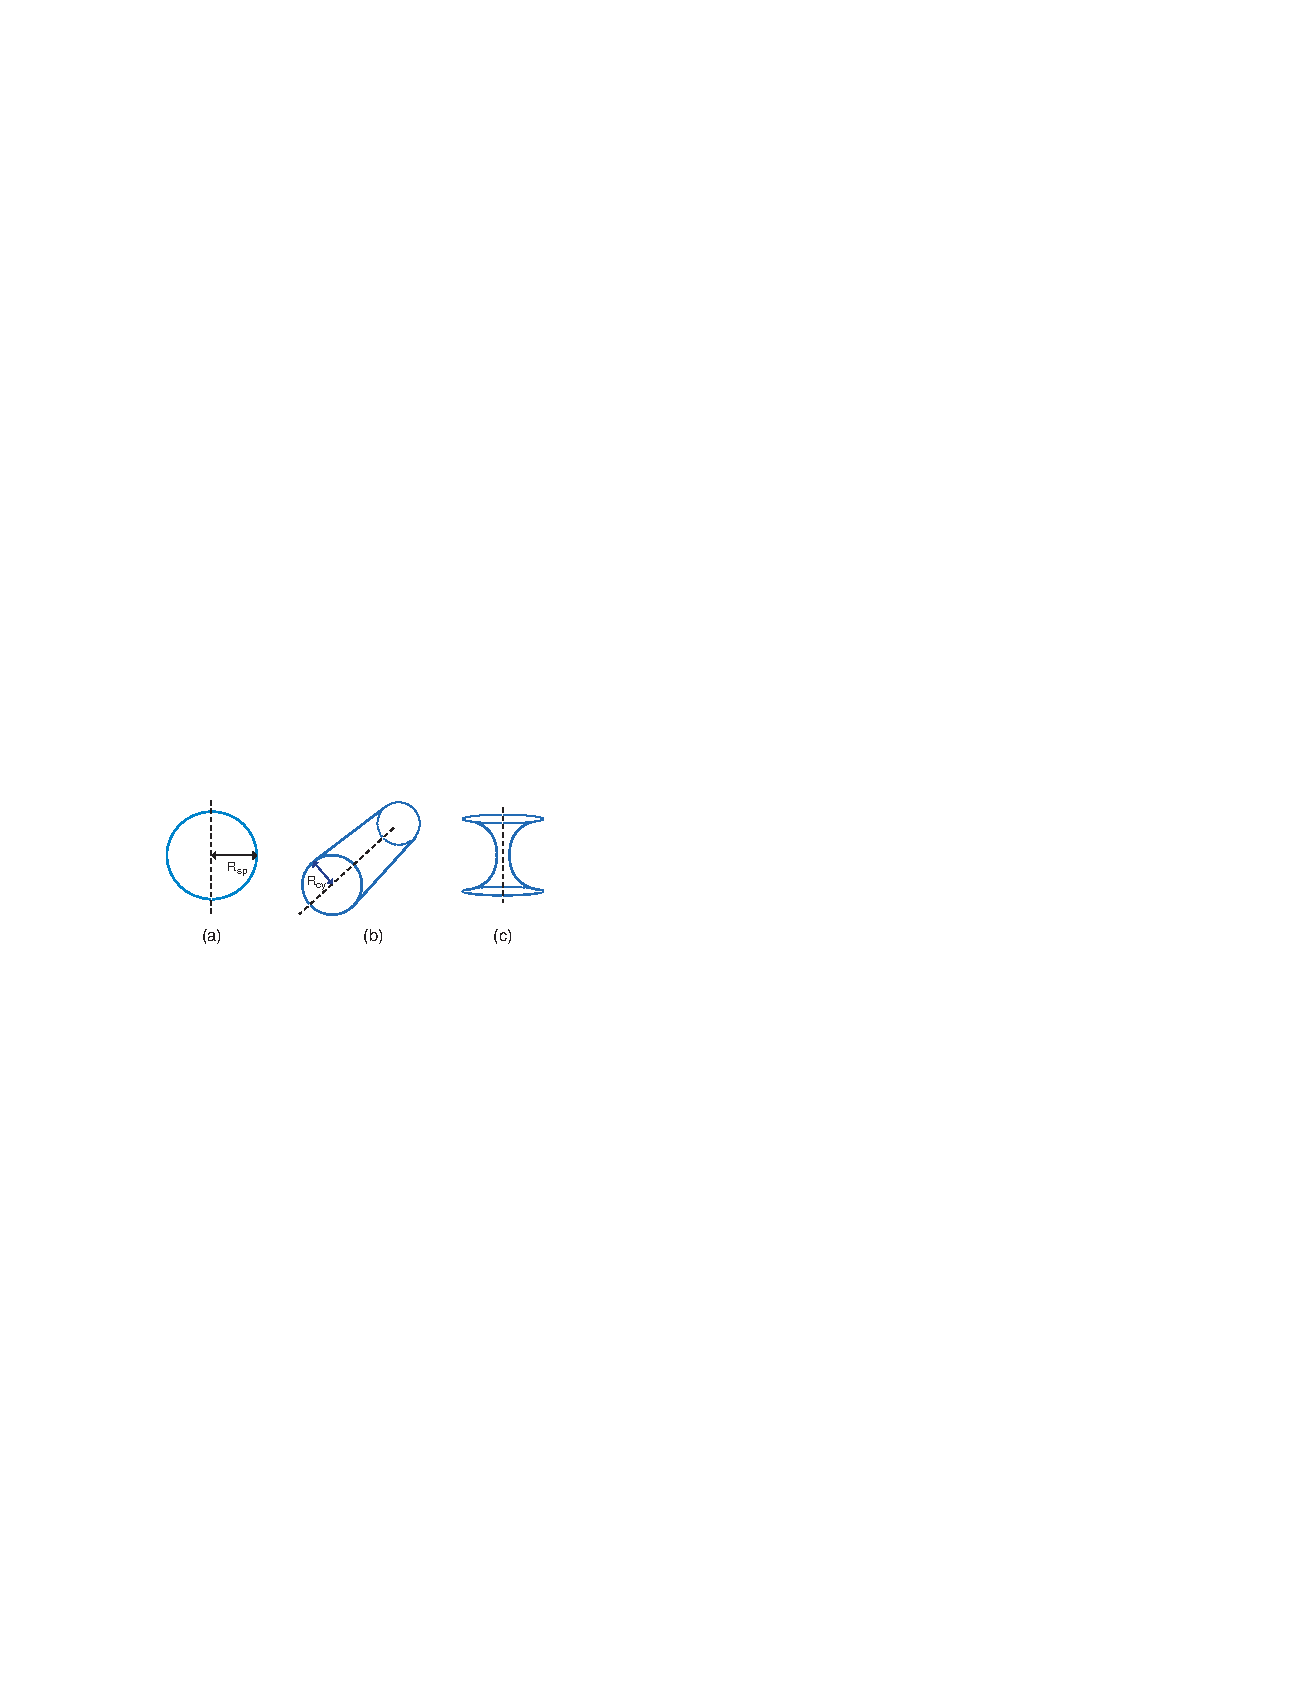
\includegraphics[width=\columnwidth]{\MemTB/Pics/simpleMembraneShapes}
\caption{
شکل‌های ساده‌ی غشا که در تمام نقاط روی سطح انحنای میانگین ثابتی دارند. شکل الف، کُره‌ای به شعاع 
$R_{sp}$
با انحنای میانگین 
$M=\pm 1/R_{sp}$
ب، استوانه‌ای با شعاع 
$R_{cy}$
با انحنای میانگین
$M=\pm 1/2R_{cy}$
و در نهایت ج، کتانوید با انحنای میانگین صفر. علامت انحنای میانگین برای کُره و استوانه به این بستگی دارد که محیط بیرون، سیال خارج از غشا تعریف شود یا سیال داخل.
}
\label{fig:simpleMembraneShapes}
\end{center}
\end{figure}
به طور عمومی انحنای میانگین یک کمیت موضعی است و در نقاط مختلف روی سطح غشا تغییر می‌کند. اما برخی اَشکال ساده در تمامی نقاط روی سطح خود یک مقدار ثابت انحنای میان‌گین دارند. برای مثال انحنای میانگین یک غشای تخت صفر است. برای مثال‌های بیشتر با شکل 
\ref{fig:simpleMembraneShapes}
توجه کنید. انحنای میانگین یک کُره با شعاع
$R_{sp}$
برابر با 
$C=1/R_{sp}$
هنگامی که لایه‌ی خارجی آن با محیط بیرون غشا در ارتباط است و 
$C=-1/R_{sp}$
زمانی که لایه‌ی داخلی آن با محیط بیرون در ارتباط است. همچنین استوانه‌‌ای با شعاع 
$R_{cy}$
دارای انحنای میانگین
$C=\pm1/2R_{cy}$
که علامت آن تابع تعریف جهت بردار عمود خواهد بود. یک شکل ساده‌ی جالب، کتانوید\LTRfootnote{catanoid} 
 است که تمام نقاط روی سطح آن از نقاط زین اسبی تشکیل شده و در نتیجه انحنای میانگین همه جا انحنای میانگین آن صفر است.





 
 
 
 
 


